\documentclass[runningheads,a4paper]{llncs}

\usepackage{graphicx}
\usepackage{wrapfig}
\usepackage{subfigure}
\usepackage[utf8]{inputenc}
\pagenumbering{roman}
\usepackage{textcomp}
\usepackage{pifont}
\usepackage{color}
\usepackage{blindtext}
\usepackage{enumitem}


\begin{document}
\mainmatter  % start of an individual contribution

%Titel
\title{HCI Meilenstein 3}

\titlerunning{HCI Meilenstein 3}

\author{
  Dursun, Camkerten
  \texttt{a0027244@@unet.univie.ac.at}
  \and
  Pektas, Tarik
  \texttt{a1325165@@unet.univie.ac.at}
  \and
  Bozkurt Yigit Berkay
  \texttt{a1029659@@unet.univie.ac.at}
  \and
  Ayyildiz Mert Ahmet
  \texttt{a1125172@@unet.univie.ac.at}
}

\institute{Universität Wien  / HCI \\
\ SS16 / Gruppe 3 (Freitag) / Team 10}


\maketitle

\section{Farbliche Analyse}
Wir haben eine ähnliche Analyse schon vor der Implementierung gemacht und konnten bei der Farbwahl uns auf Farben beschränken welche auch von Farbblinden Menschen einwandfrei wahrgenommen werden können. Eine entsprechende Analyse in der wir den Color Blindness Simulator von Coblis verwendet haben bestätigte uns die von uns bereits erwarteten Resultate[1].\\ \\ 
Was allerdings leider nicht so gut funktioniert hat, war die Analyse der Reporting Seite da wir uns für eine Pie Chart entschieden hatten.\\\\ Da dieser sehr viele Farben, basierend auf unterschiedliche Datentypen hat, kann man da auch nicht viel ausrichten.\\ Dennoch haben wir, um den Informationsfluss auf jeden Fall zu gewähren, alternative Typen implementiert, wie zum Beispiel Table Chart oder Line Chart, welche die entsprechenden Farbanalysen bestanden haben und somit von jedem wahrgenommen werden können.

\begin{figure}
\centering
\subfigure[Normal Color Vision]{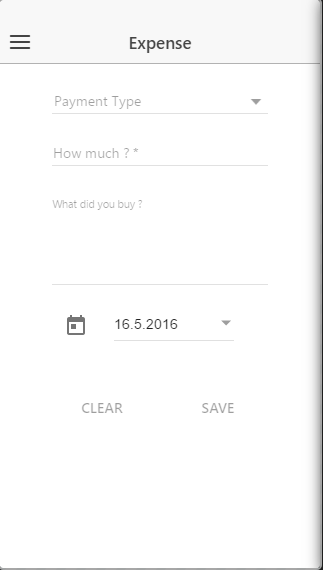
\includegraphics[width=0.15\textwidth]{expense.png}}
\hfill
\subfigure[Blue-Blind/Tritanopia]{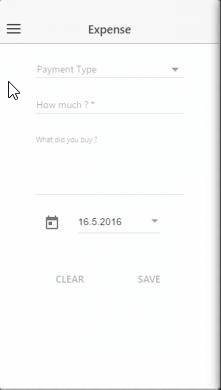
\includegraphics[width=0.15\textwidth]{expenseBlueBlind.png}}
\hfill
\subfigure[Green-Blind/Deuteranopia]{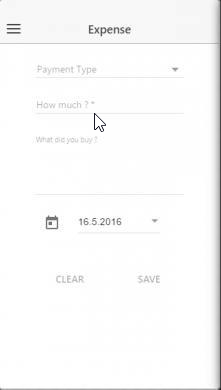
\includegraphics[width=0.15\textwidth]{expenseGreenBlind.png}}
\hfill
\subfigure[Red-Blind/Protanopia]{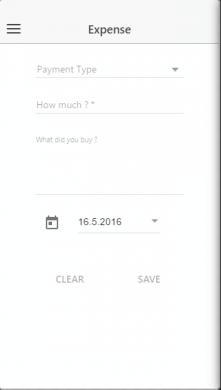
\includegraphics[width=0.15\textwidth]{expenseredblind.png}}
\end{figure}


\clearpage


\begin{figure}
\centering
\subfigure[Normal Color Vision]{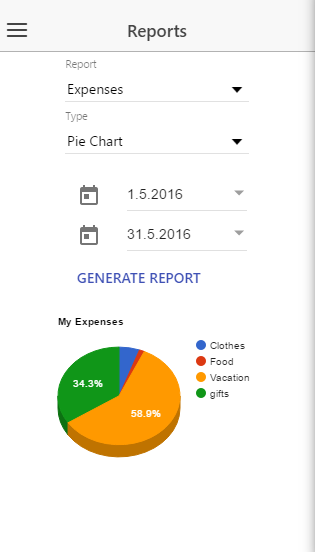
\includegraphics[width=0.15\textwidth]{ReportPieChart}}
\hfill
\subfigure[Blue-Blind/Tritanopia]{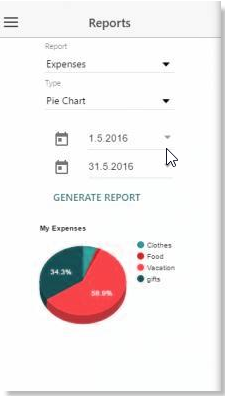
\includegraphics[width=0.15\textwidth]{ReportPieChartA2blueBlind.png}}
\hfill
\subfigure[Green-Blind/ Deuteranopia]{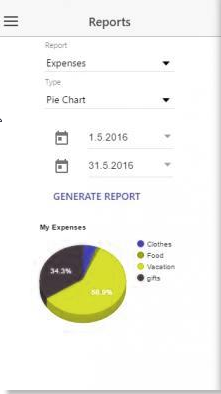
\includegraphics[width=0.15\textwidth]{ReportPieChartA2greenBlind.png}}
\hfill
\subfigure[Monochromacy/ Achromatopsia]{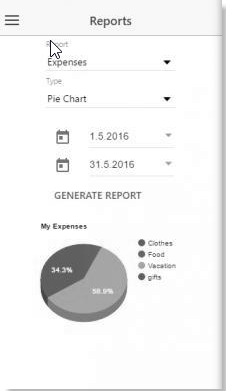
\includegraphics[width=0.15\textwidth]{ReportPieChartA2monochrom.png}}
\hfill
\subfigure[Red-Blind/Protanopia]{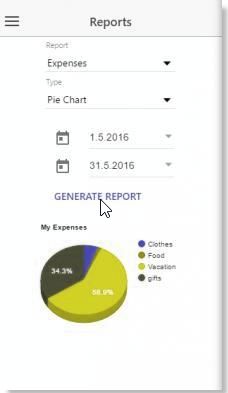
\includegraphics[width=0.15\textwidth]{ReportPieChartA2redBlind.png}}
\end{figure}

\begin{figure}
\centering
\subfigure[Normal Color Vision]{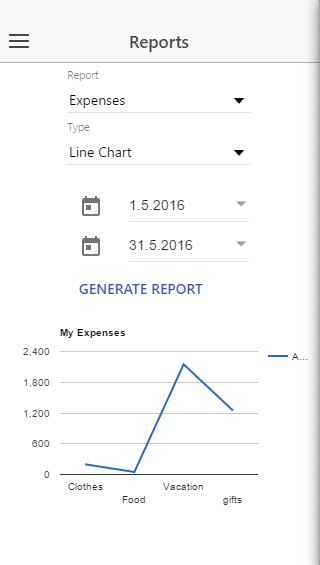
\includegraphics[width=0.15\textwidth]{LineChart.png}}
\hfill
\subfigure[Normal Color Vision]{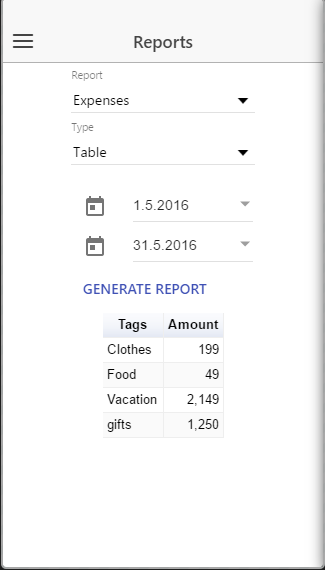
\includegraphics[width=0.15\textwidth]{tableChart.png}}
\hfill
\subfigure[Blue-Blind/Tritanopia]{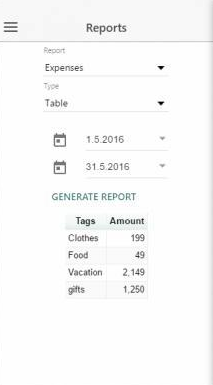
\includegraphics[width=0.15\textwidth]{tableChartBlueBlind.png}}
\hfill
\subfigure[Green-Blind/ Deuteranopia]{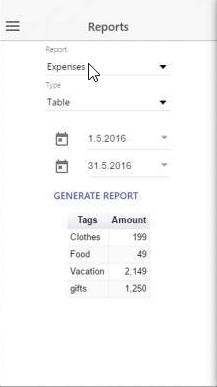
\includegraphics[width=0.15\textwidth]{tableChartGreenBlind.png}}
\hfill
\subfigure[Red-Blind/Protanopia]{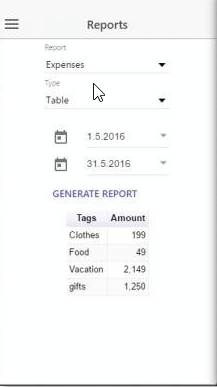
\includegraphics[width=0.15\textwidth]{tableChartRedBlind.png}}
\end{figure}




\section{Kognitive Analyse}

\subsection{Fitts Law und Hicks Law}

Wir haben versucht die gleichen Datentypen bzw Eingabefelder, wie zum Beispiel; Datum der Ausgabe; Startdatum für das Reporting, Datum der Einnahme etc. immer an die gleiche Stelle zu positionieren.\\\\  Dies galt natürlich auch für die restlichen Eingabefelder. Wir denken, dass wir somit eine Konsistenz in Bezug auf, häufig gesuchte Ziele an der gleichen Stelle, erstellen konnten. Bezüglich der Größe denken wir dass unsere Auswahl an Font und Size intuitiv bereits mit Fitts Law konform war.\\\\   Lag wahrscheinlich daran das bei Mobile Apps grundsätzlich Ziele des Öfteren sehr groß dargestellt werden. Wir beschlossen außerdem keine verschachtelten Menüstrukturen zur erstellen. \\\\ Alle wählbaren Optionen wurde in einzelnen Drop Down Menü Boxen erstellt.  Die Auswählbaren alternativen wurden in ihrer einfachsten Form, (Expense, Income, Report), formuliert. 


\begin{figure}
\centering
\subfigure[Expense]{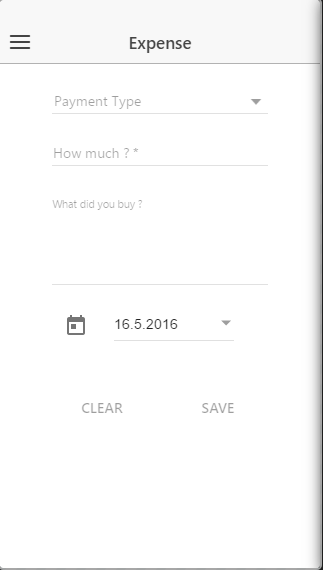
\includegraphics[width=0.15\textwidth]{expense.png}}
\hfill
\subfigure[Income]{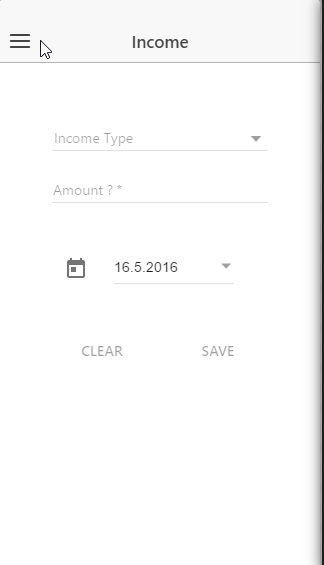
\includegraphics[width=0.15\textwidth]{income.png}}
\hfill
\subfigure[Report]{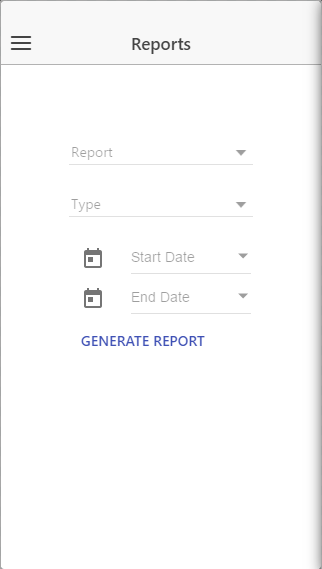
\includegraphics[width=0.15\textwidth]{Report.png}}
\end{figure}


\section{Prototyp Beschreibung}

\clearpage

\begin{thebibliography}{1}
\bibitem{proceeding1} http://www.color-blindness.com/coblis-color-blindness-simulator/
\end{thebibliography}


\end{document}